% ---------------------------------------------------------------------
\subsection{Covariance Estimation}\label{subsec:rcc-local}\label{subsec:ruido-colorido}\label{subsubsec:estimacao-R}
% ---------------------------------------------------------------------
The BS knows the channel matrix $\mathbf H$ of its UEs, but it does not know the matrix $\overline{\mathbf H}$ of the non-target UEs nor the power $\beta$ with which they transmit. Therefore, the BS estimates $\mathbf R_n$ by averaging $N$ samples of noise it receives \cite{tomasin-interference}:


\begin{equation}\label{eq:Rn_est}
\widehat{\mathbf R}_n=
\frac{1}{N}
\sum_{i=1}^{N}
\mathbf n^i(\mathbf n^i)^H,
\end{equation}


where $\mathbf n^i\in\mathbb C^{M\times1}$ is the noise sample in the $i$-th pilot RE, reference REs that the UEs transmit to the BS to estimate the channel \cite{marzetta2016fundamentals}. The receiver knows the pilot of the target UEs and can remove it from the received signal. What remains is interference plus thermal noise. Each element of $\mathbf n^i(\mathbf n^i)^H$ is the product $n_a^i(n_b^i)^*$ between the noise of two antennas. The diagonal elements ($a=b$) are the power in one antenna. The average of these products estimates each element of $\mathbf R_n$. The receiver performance improves with the number of samples $N$ \cite{tomasin-interference}.
% FONTE: Marzetta et al., Seção 3.1, p. 45.
% FONTE: tomasin-interference p. 1773, Eq. 6; Figs. 5 e 6.

In the decentralized uplink, each noise sample is also divided between the clusters, $\mathbf n^i = [(\mathbf n_1^i)^T, \ldots, (\mathbf n_C^i)^T]^T$, and the DU $c$ only keeps its part. Likewise, $\mathbf R_n$ becomes \textcolor{red}{a matrix} of $C \times C$ blocks\textcolor{red}{. The block $\mathbf R_{\mathrm{row},\mathrm{col}} = \mathbb E[\mathbf n_{\mathrm{row}}\mathbf n_{\mathrm{col}}^H]$ relates the noise of the antennas of cluster $\mathrm{row}$ to the noise of the antennas of cluster $\mathrm{col}$ (Figure~\ref{fig:rn-blocos})}. Each DU can only estimate its diagonal block with its own samples \textcolor{red}{\cite{zhao2021-globecom,zhao2025jsac}}:

% FONTE: zhao2021-globecom L88 e L90.
\begin{equation}
\hat{\mathbf R}_{cc}=
\frac{1}{N}
\sum_{i=1}^{N}
\mathbf n_c^i(\mathbf n_c^i)^H.
\label{eq:Rcc_est}
\end{equation}

Off-diagonal blocks, \textcolor{red}{$\mathbf R_{\mathrm{row},\mathrm{col}}$ with $\mathrm{row} \neq \mathrm{col}$}, combine the noise from two clusters. To estimate them, the DUs would have to exchange $N$ samples for each of the $M$ antennas, which is not feasible in massive MIMO. Therefore, BCD-MMSE does not exchange samples. Each DU uses only the samples from its cluster and passes the results $\mathbf A_c$ and $\mathbf b_{c,i}$ to the next DU in the chain (\textcolor{red}{Figure~\ref{fig:bcd-etapas}(b)} and Section~\ref{subsec:bcd}). The size of these results depends on the number of UEs $K$, and not on the number of antennas $M$ \cite{zhao2025jsac}.

% FONTE: zhao2025jsac paper.md:39-41, :125, :130 e :571.

\begin{figure}[!ht]
\caption[Blocks of $\mathbf R_n$.]{Blocks of $\mathbf R_n$, with $C \times C$ blocks of $M_c \times M_c$ elements. In red, the blocks that DU 3 needs.}
\label{fig:rn-blocos}
\vspace{4pt}
\centering
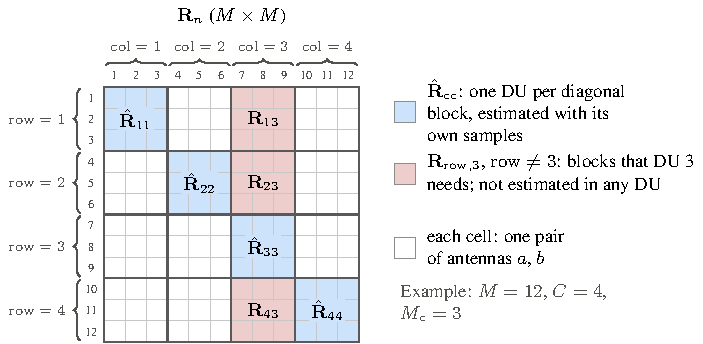
\includegraphics{Images/FLUXO/rn_blocos.pdf}
\vspace{4pt}
\legend{Source: adapted from \citesp{zhao2025jsac}.}
\end{figure}
% FONTE: zhao2025jsac, Fig. 3 (paper.md:127-128) e Algoritmo 3.
